%%%%%%%%%%%%%%%%%%%%%%%%%%%%%%%%%%%%%%%%%%%%%%%%%%%%%%%%%%%%%%%%%%%%%%%%%%%%%%%
\section{Aberration Measurement and Correction}
\label{Measurement}
%%%%%%%%%%%%%%%%%%%%%%%%%%%%%%%%%%%%%%%%%%%%%%%%%%%%%%%%%%%%%%%%%%%%%%%%%%%%%%%

%explain what are abberations, how they arrise, why it is good to correct them
%I just proposed a rough structure, but I am realizing now, that all the 
%sub-sub-section will take up a lot of room. so it might be better if you 
%remove them an explain it all in one subsection
%here is some stuff that I collected/copied from the paper you gave me

For the purpose of understanding the operation of an adaptive optical system, 
it is best to think of aberrations in terms of distortions of an optical 
wavefront.

\begin{figure}[tbh]
        \centering
        \begin{subfigure}[b]{0.4\textwidth}
                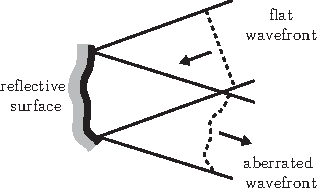
\includegraphics[width=\textwidth]{images/wavefront_distortions_reflection}
                \caption{Reflection.}
                \label{fig:abberation_reflection}
        \end{subfigure}
				\hspace{1em}
        \begin{subfigure}[b]{0.3\textwidth}
                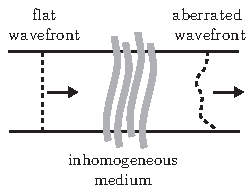
\includegraphics[width=\textwidth]{images/wavefront_distortions_transmission}
                \caption{Transmission.}
                \label{fig:abberation_trans}
        \end{subfigure}
        \caption{Wavefront aberrations due to (a) reflection from a non 
planar surface and (b)  caused by propagation through a non-uniform 
refractive index distribution. Image after~\cite{book_aberrations}.}
\label{fig:abberations}
\end{figure} 

Representing aberrations in this way can simplify the design, control and 
characterisation of adaptive optics. The choice of modes for a particular 
application is often influenced by some aspect of the system, such as the 
deformation modes of a deformable mirror or the statistics of the induced 
aberrations. Otherwise, the modal representation may be chosen through 
mathematical convenience. For example, Zernike polynomials are often used for 
systems with circular apertures as they form a complete, orthogonal set of 
functions defined over a unit circle

As with all optical systems, microscopes can also suffer from aberrations due 
to imperfections in the optical components. In practice, no system can be 
totally free from aberrations and so systems are designed to maintain 
aberrations below a particular tolerance for a given set of imaging 
conditions, such as wavelength, magnification and field of view. Significant 
aberrations can be introduced if a microscope is used outside its design 
specifications, for example at the incorrect wavelength or at a difierent 
temperature (see Chapter 11 of Ref. 9).

\cite{AOM_basic_ref}


%%%%%%%%%%%%%%%%%%%%%%%%%%%%%%%%%%%%%%%%%%%%%%%%%%%%%%%%%%%%%%%%%%%%%%%%%%%%%%%
\subsection{Direct Wavefront Sensing}
\label{sec:WavefrontSensing}

%------------------------------------------------------------------------------
\subsubsection{Lateral Shearing Interferometer}
\label{sec:DirectWavefrontSensing_interferometry}
%not sure if this is used for microscopy, we should at least mention it

%------------------------------------------------------------------------------
\subsubsection{Shack-Hartman Wavefront Sensor}
\label{sec:DirectWavefrontSensing_SHWS}

%------------------------------------------------------------------------------
\subsubsection{Curvature Sensor}
\label{sec:CurvatureSensor}


%%%%%%%%%%%%%%%%%%%%%%%%%%%%%%%%%%%%%%%%%%%%%%%%%%%%%%%%%%%%%%%%%%%%%%%%%%%%%%%
\subsection{Indirect Wavefront Sensing}
\label{sec:IndirectWavefrontSensing}

While direct wavefront sensing techniques are widely applied in Astronomy, 
they are less common in microscopy techniques. This for several reasons. It 
is not as easy to create a guiding start like point source in a biological 
specimen. If there are not features in the specimen that occur there 
naturally and which resemble a point source, one has to be implemented 
manually which might alter the function of the specimen or might even be 
toxic to the sample. Modern microscopes are also highly complex and 
optimized, which makes it difficult to insert a relatively large wavefront 
sensor. For samples with weak signal strength, it is also desirable to 
collect as many photons as possible for the imaging process. Splitting the 
beam and using a part of the light emitted from the sample for direct 
wavefront sensing might hence decrease the signal strength too much.

Indirect techniques do not measure the wavefront directly but instead 
optimize the image quality. This leads to the retrieval of the aberration and 
the necessary corrections. Hence these techniques don't sense the wavefront 
but rather improve the image quality and through this correct for wavefront 
aberrations. Indirect methods are used more often in industrial and medical 
applications. They usually require very little additional hardware. Once the 
technique is optimized for a specific problem, indirect schemes are easier to 
implement in practice and are more prone to errors due to the lack of 
additional hardware~(a single deformable mirror might be sufficient to 
implement adaptive optics in an existing microscope). 

Indirect techniques include phase diversity as well as optimization of an 
image quality metric. Phase diversity techniques use two or more images of an 
extended object to make an estimation of the distorting 
wavefront~\cite{indirect_phase_retrieval_algorithm}. However, this technique 
still requires 
a beam splitter, a second detector and a deformable mirror which is a 
significant disadvantage over image quality metric optimization where only 
the normally recorded image and a deformable mirror is required. It is also 
necessary to record images with different focus positions and hence the each 
phase retrieval step takes many seconds. Therefore the entire process of 
optimizing the wavefront takes minutes, which is to slow for most biological 
imaging~\cite{indirect_AOM_phase_retrieval}. It is for these reasons that 
phase diversity techniques are less common in microscopy and will not be 
described further. The focus of this section is therefor a general 
description of image quality metric techniques. Their specific properties and 
how they are implemented in the different microscopy techniques is then 
described in Section~\ref{sec:ExperimentDiscussion}.

%------------------------------------------------------------------------------
%Optimization of an Image Quality Metric

The optimization of an image quality metric is mainly a mathematical rahter then a techniquel problem. We will describe the basic principle but the derivation of the specifc metrics is beyond the scope of this paper. The interested reader will find more information on the mathematical background in reference~\cite{wide_parabolic_optimization,wide_sphere_packing,wide_Lukosz_Modes,wide_AOM_loew_freq}. 

For these techniques, the aberration correction is performed through an iterative optimization of an image quality metric based. The metric is usually based on spatial frequencies~\cite{wide_AOM_loew_freq} or image intensity~\cite{indirect_metric_intensity}. Such optimization is either implemented empirically or by using an appropriate mathematical model. In many practical systems aberrations can be accurately represented by a small number of modes of an orthogonal basis, such as Zernikepolynomials. A sequence of images is acquired, each with a different aberration applied and the correction aberration is estimated from the information in this images. This process is repeated until the image quality is considered acceptable. The number of measurements needed to obtain an acceptable image depends strongly upon the optimization algorithm and parameters used, the mathematical representation of the aberration, and the object structure. For the earliest and most generic algorithms the number of measurements per aberration mode increases quadratically or exponentially with $N$, the number of corrected aberration modes~\cite{wide_sphere_packing}. The so called direct maximization method~(as described in Section~\ref{sec:TransmissionMicroscope}) is significantly more efficient, requiring only $N+1$ measurements for $N$ mode. With this technique, Lukosz polynomials~\cite{wide_Lukosz_Modes} are used to clasify the aberrations. The effects of different modes can then be separated and the optimization of each mode becomes independent and hence more efficient.

An effective model-based adaptive optics scheme should also be independent of the imaged object and should permit the separation of aberration and object influences on the measurements. This separation is also possible through the appropriate choice of optimization metric and aberration representation~\cite{wide_AOM_loew_freq}.


%%%%%%%%%%%%%%%%%%%%%%%%%%%%%%%%%%%%%%%%%%%%%%%%%%%%%%%%%%%%%%%%%%%%%%%%%%%%%%%
\subsection{Aberration Correction}
\label{sec:AberrationCorrection}
% just mention the basic principles, i.e. liquid crystal, deformable mirror, 
%computational

%------------------------------------------------------------------------------
\subsection{Deformable Mirrors}
\label{sec:DeformableMirror}

%------------------------------------------------------------------------------
\subsubsection{Liquid Crystal Spatial Light Modulators}
\label{sec:LiquidCrystalSpatialLightModulators}
% I used Nematic Liquid Crystalls for my Bachelor Thesis, so if you need 
% infos or graphs about them, let me know and I might be able to help

%%%%%%%%%%%%%%%%%%%%%%%%%%%%%%%%%%%%%%%%%%%%%%%%%%%%%%%%%%%%%%%%%%%%%%%%%%%%%%%
\subsection{Control Strategies}
\label{sec:ControlStrategies}

\clearpage